\section{Introduction}
\label{sec:intro}

In recent years, there has been a significant surge in the capabilities of large language models (LLMs) in generating human-like text and performing a wide range of natural language processing tasks. State-of-the-art models like GPT-4o~\citep{Hurst2024GPT4oSC}, OpenAI o1/o3~\citep{Contributors2024OpenAIOS}, and Google's Gemini~\citep{team2023gemini} have achieved superior performance in knowledge QA~\citep{Hendrycks2020MeasuringMM,Wang2024MMLUProAM}, instruction-following~\citep{Chiang2024ChatbotAA,Zhou2023InstructionFollowingEF}, and code generation~\citep{Zhuo2024BigCodeBenchBC,Jain2024LiveCodeBenchHA}.

Despite recent advances, many real-world applications require not only fluency in the content of the output but also precise control over its structure. This includes tasks where the expected output must follow specific formats such as JSON, XML, LaTeX, HTML, or code in frameworks like React or Vue. Additionally, in these tasks, in these tasks, we also want the code to render a page that correctly places elements according to the requirements. These types of structured output are essential in domains like software development, data pipelines, user interface generation, and scientific publishing, where incorrect formatting can lead to disrupted pipelines or non-functional outputs.

% \begin{figure}
%     \centering
%     \includegraphics[width=0.5\linewidth]{}
%     \caption{Caption}
%     \label{fig:enter-label}
% \end{figure}
% \begin{figure}
%     \centering
%     \fbox{\phantom{\rule{\linewidth}{1.0\linewidth}}}
%     \caption{\structeval evaluates the LLM's capability to generate structured outputs, including text-only tasks like JSON, TOML, etc, and visual rendering tasks like HTML, React, Latex, etc.}
%     \label{fig:enter-label}
% \end{figure}

\begin{figure}[t]
    \centering
    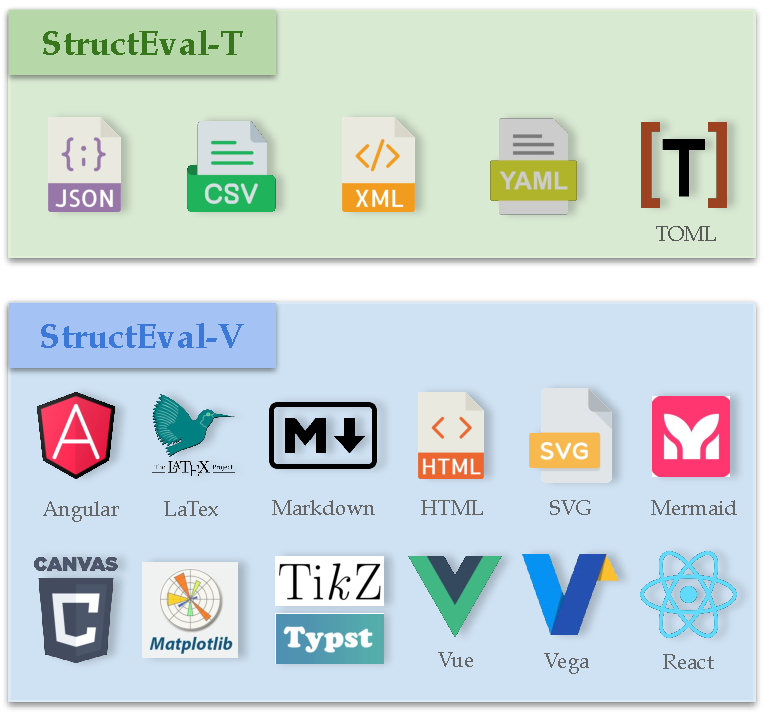
\includegraphics[width=0.98\linewidth]{./figures/intro.pdf}
    \caption{\structeval evaluates the LLM's capability to generate structured outputs, including text-only tasks like JSON, TOML, etc, and visual rendering tasks like HTML, React, Latex, etc.}
    \label{fig:intro}
\end{figure}
% \begin{figure}
%     \centering
%     \includegraphics[width=0.5\linewidth]{}
%     \caption{Caption}
%     \label{fig:enter-label}
% \end{figure}
\begin{figure*}[!t]
    \centering
    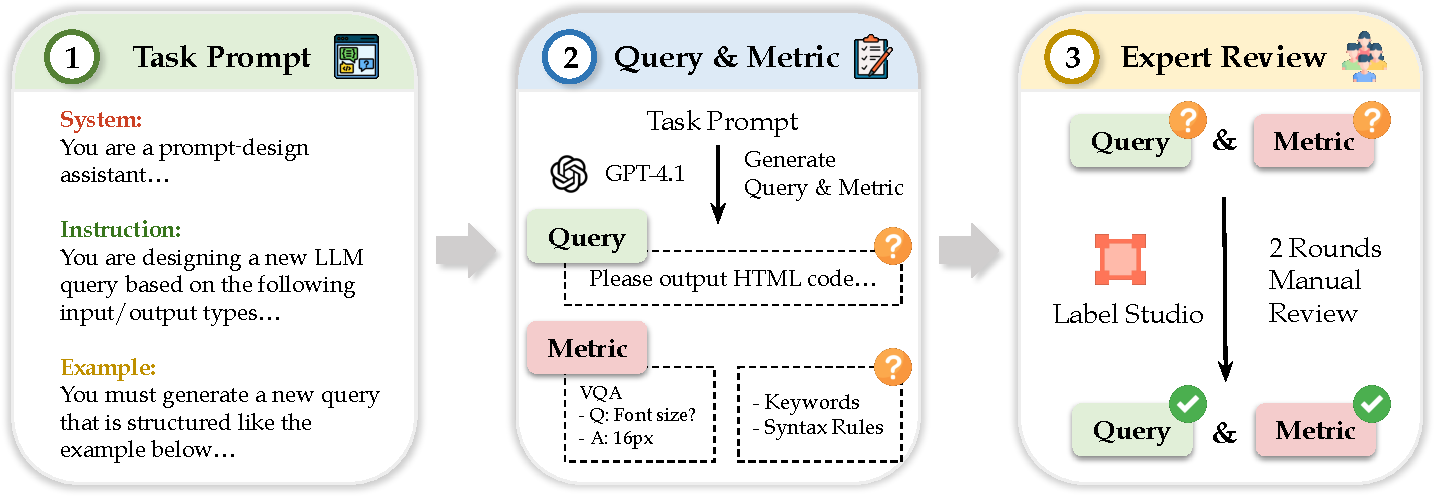
\includegraphics[width=1\linewidth]{./figures/annotation_pipeline.pdf}
    \caption{The overall designed annotation pipeline of \structeval dataset}
    \label{fig:annotation_pipeline}
\vspace{-1em}
\end{figure*}

However, most existing benchmarks focus on the semantic quality~\citep{Wang2024MMLUProAM} or reasoning ability of LLMs~\citep{Hendrycks2021MeasuringMP,He2024OlympiadBenchAC}, with limited emphasis on their ability to produce format-conforming structured outputs. Some recently proposed benchmarks aim to evaluate the quality of structured outputs tend to target specific modalities, such as code generation~\citep{Zhuo2024BigCodeBenchBC} or text-only structures~\citep{gu2024structext,tang-etal-2024-struc}, rather than offering comprehensive evaluations across diverse structured formats. As existing benchmarks gradually become more saturated, it is still unknown how the current state-of-the-art models perform in structured generation tasks. We argue that effectively evaluating the models' performance on such tasks is inherently challenging due to the following issues:



\noindent \textbf{(1) Data Collection Challenges:} Gathering diverse structured tasks and corresponding examples requires domain expertise across multiple formats, with high-quality annotations demanding significant effort and specialized knowledge.

\noindent \textbf{(2) Evaluation Metric Complexity:} Designing reasonable metrics in a unified form for both text-only structures (JSON, YAML) and visual outputs (HTML, SVG) is difficult, as they require different assessment approaches for structural correctness and visual fidelity.

\noindent \textbf{(3) Technical Implementation Barriers:} Building a framework that supports execution and evaluation across numerous rendering environments requires complex integration of multiple language interpreters and visualization tools.

To address these challenges, we introduce \textsc{StructEval}, a comprehensive benchmark that systematically evaluates LLMs' abilities to produce highly structured output. Our benchmark encompasses 21 distinct formats and 44 task types organized into two complementary subsets: \emph{StructEval-T}, which assesses the generation of text-only structures such as JSON and TOML, and \emph{StructEval-V}, which evaluates the quality of visually rendered outputs from code such as HTML and SVG. Both subsets include generation tasks (converting natural language to structured outputs) and conversion tasks (transforming between two structured formats). To ensure robust evaluation across these diverse formats, we have developed a novel assessment framework that integrates syntactic validity checking, keyword matching, and visual question answering, providing a holistic measure of both structural correctness and output fidelity.


Our comprehensive evaluation reveals significant performance gaps across models and tasks. Even state-of-the-art commercial models like o1-mini achieve only an average score of $75.58$, while the best open-source model, such as Llama-3-8B-Instruct, lags $10$ points behind, underscoring the performance gap between commercial and open-source LLMs. We observe that generation tasks generally pose greater challenges than conversion tasks, and producing code capable of rendering correct visual content proves more difficult than generating text-only structured outputs. Task difficulty varies considerably across formats: while some tasks are effectively solved by all LLMs with scores exceeding $0.95$ (such as Text$\rightarrow$Markdown and Text$\rightarrow$HTML), others remain particularly challenging with all models scoring below $0.5$ (including Text$\rightarrow$Mermaid and Matplotlib$\rightarrow$TikZ). Through this systematic analysis, we aim to drive progress in structured output generation capabilities that are increasingly crucial for the real-world applications of language models.